\section{Problem Description}\label{sec:prob_descr}

The purpose of this report is to show how an error-state Kalman filter (ESKF)
can utilize IMU and GNSS measurements to track a flying object. 
For this we are given two datasets.
The first dataset is simulated and includes a truth value,
this allows for calculation of Normalized Estimation Error Squared (NEES) values,
to tune with regards to estimation error.
For both datasets we can compute Normalized Innovation Squared (NIS) to tune 
with regards to error in the innovation.

\section{ESKF}\label{sec:eskf}



\section{Tuning}\label{sec:tuning}

\subsection{Process}

The initial parameters, based on the sampling time and expected 
noise of the sensor and the sampling time, provided a good starting point.
What was lacking appeared to be an ability of the system to make proper turns.
A possible explanation is that the calculated noises dont account for
any significant maneuvering. 
The noises should therefore be slightly increased in order for the filter
to also account for reasonable changes in attitude and position.
NEES values for the individual gyroscope and accelerometer axes 
were also used for more detailed tuning.
A short outline of the initial tuning process is listed here along with a discussion below.

\begin{enumerate}
	\item Tune measurement noise until the GNSS track is followed
	\item Tune process noise to get a decent result from NEESes
	\item Tune IMU bias driving noises to reduce trends in gyro and acceleration NEES bias
	\item Tune individual measurement and process noise parameters to fit individual IMU NEES axis in the middle of interval
\end{enumerate}

An observation made was that certain larges deviations occured in the NEESes. 
This appears to be due to larger then normal changes in position and attitude. 
Due to the infrequent GNSS updates, the process noise was increased while
the measurement noises was decreased to try to better account for these occurrences.
The reasoning being that the IMU might be able track the true value better.
Reducing measurement noise in favour of process noise also improved NIS results, 
by reducing overfitting in parts of the track. 

The tuning appeared in large part to be a bias-variance tradeoff problem.
Our experience was that reducing the variance during fast maneuvers led to overfitting elsewhere.
Likewise acceptable bias-variance on most of the track tended to cause underfitting during fast maneuvers.
From a practical point of view we would argue that it makes more sense to track the harder parts better
and accept some overfitting elsewhere if the alternative is to have huge errors in certain parts of the track.
There is ofcourse a tradeoff and 

\begin{tabular}{ |p{5cm}||p{3cm}|p{3cm}|  }
	\hline
	\multicolumn{3}{|c|}{Results} \\
	\hline
	Parameter & Simulated data & Real data\\
	\hline
	NIS mean				& 1.4971  	&   004\\
	NEES tot mean			& 13.0695 	&	248\\
	NEES pos mean 			& 1.4101 	&  008\\
	NEES vel mean			& 0.9584 	& 012\\
	NEES att mean			& 0.9281 	& 016\\
	NEES acc bias mean		& 5.3252 	& 020\\
	NEES gyro bias mean 	& 0.9258 	& 024\\
	Estimated pos RMSE		& 0.5637 	& 024\\
	Estimated vel RMSE		& 0.3485 	& 024\\
	Measured pos RMSE		& 0.6735 	& 024\\
	\hline
   \end{tabular}


\begin{figure}
    \centering
    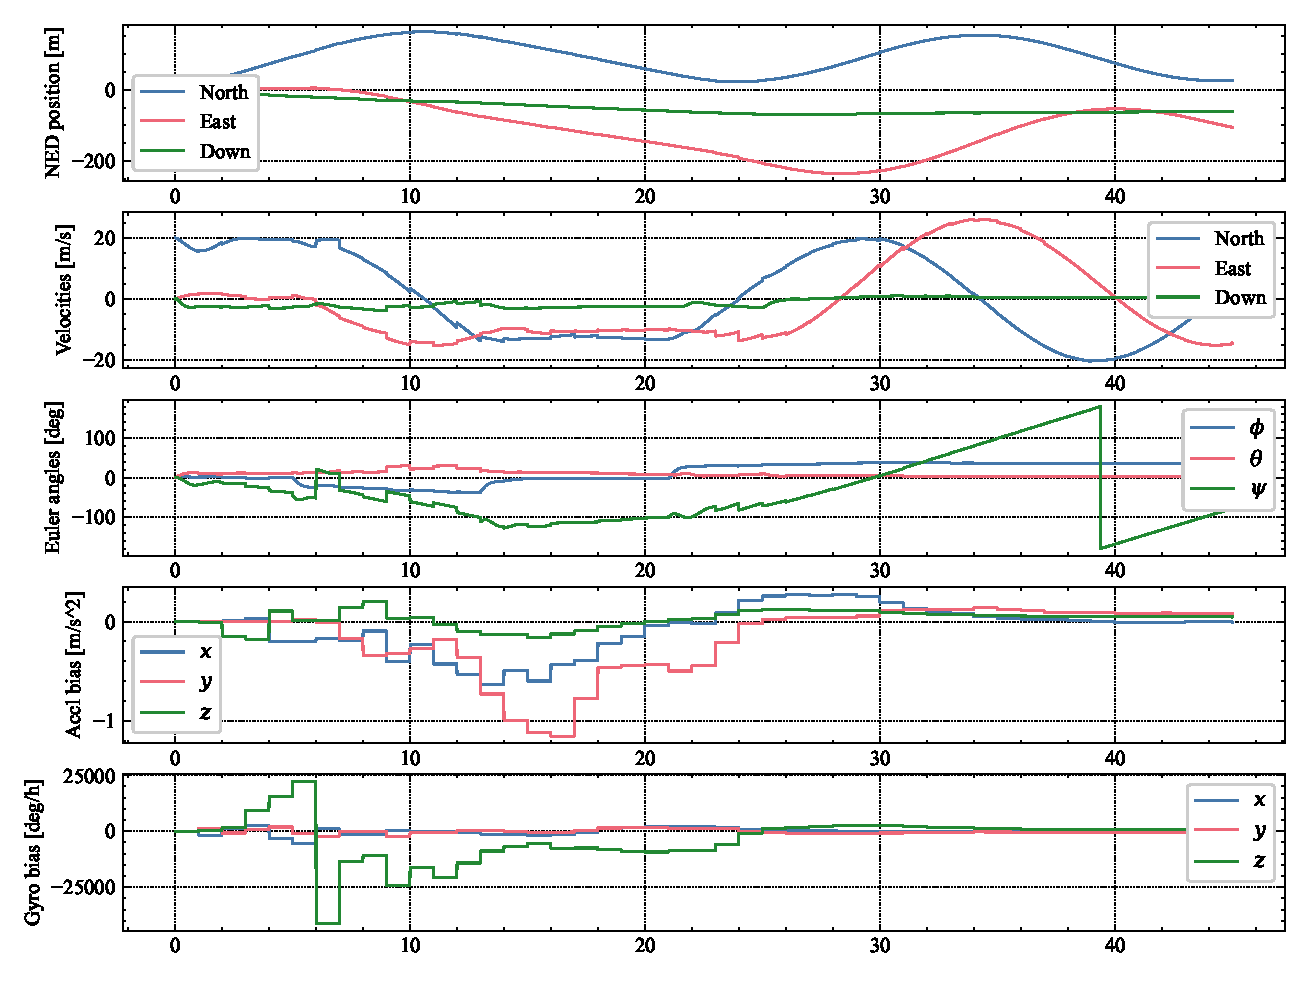
\includegraphics[clip, trim= 0cm 0cm 0cm 0cm, width = \textwidth]{figures/sim_2.eps}
    \caption{Estimated states}
    \label{fig:1_2}
\end{figure}
\begin{figure}
    \centering
    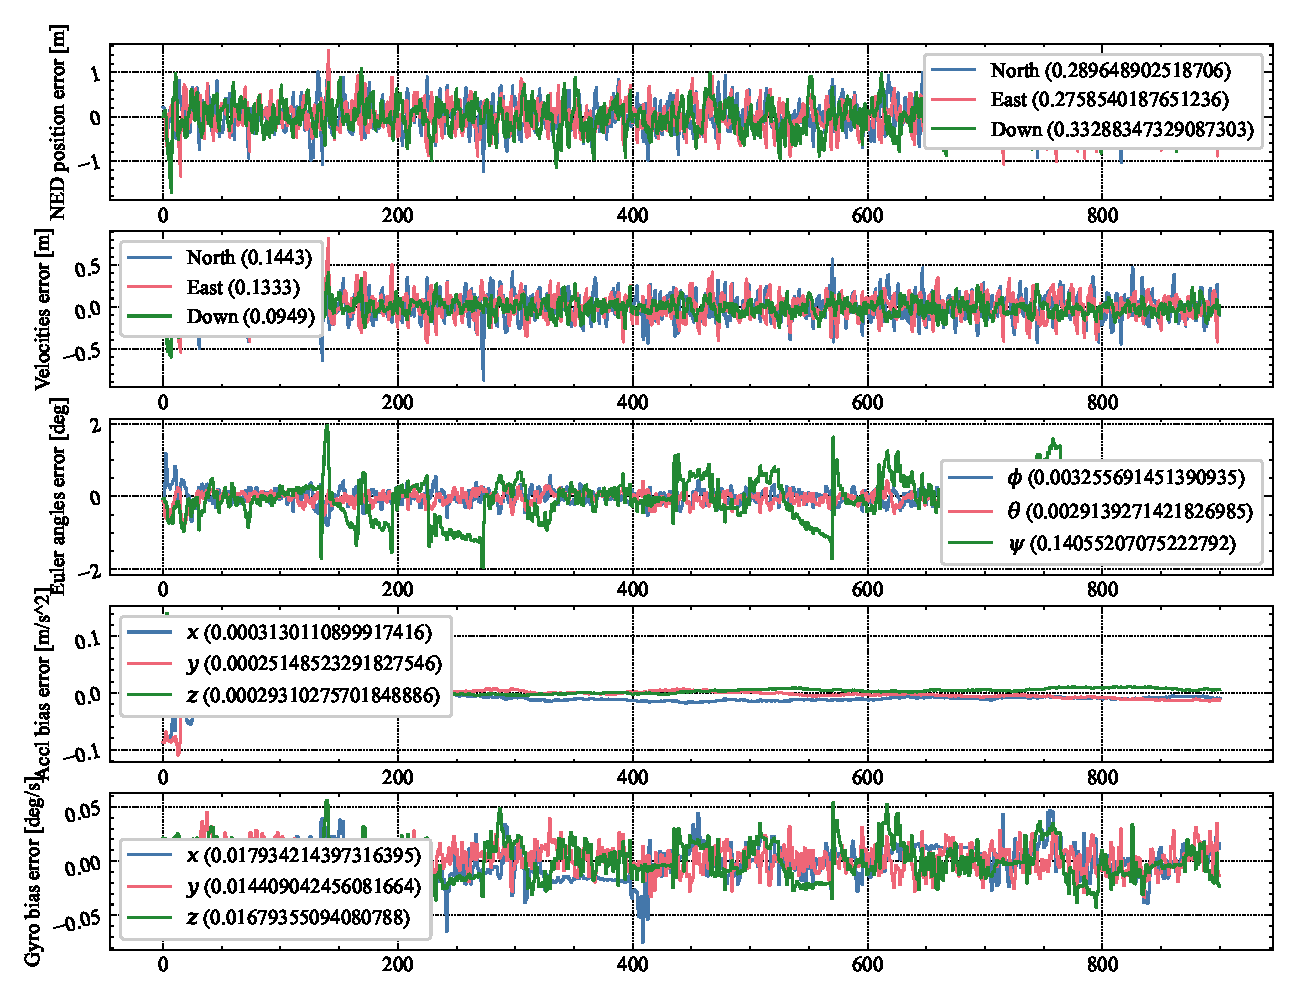
\includegraphics[clip, trim= 0cm 0cm 0cm 0cm, width = \textwidth]{figures/sim_3.eps}
    \caption{True error states}
    \label{fig:23states}
\end{figure}
\begin{figure}
    \centering
    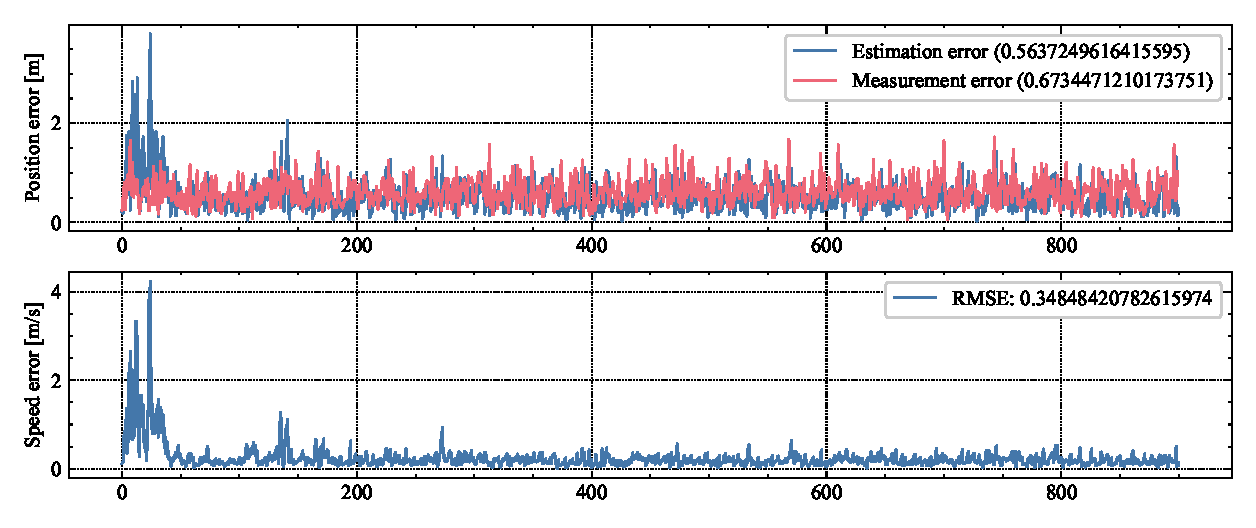
\includegraphics[clip, trim= 0cm 0cm 0cm 0cm, width = \textwidth]{figures/sim_4.eps}
    \caption{Error distance}
    \label{fig:23state_error}
\end{figure}
\begin{figure}
    \centering
    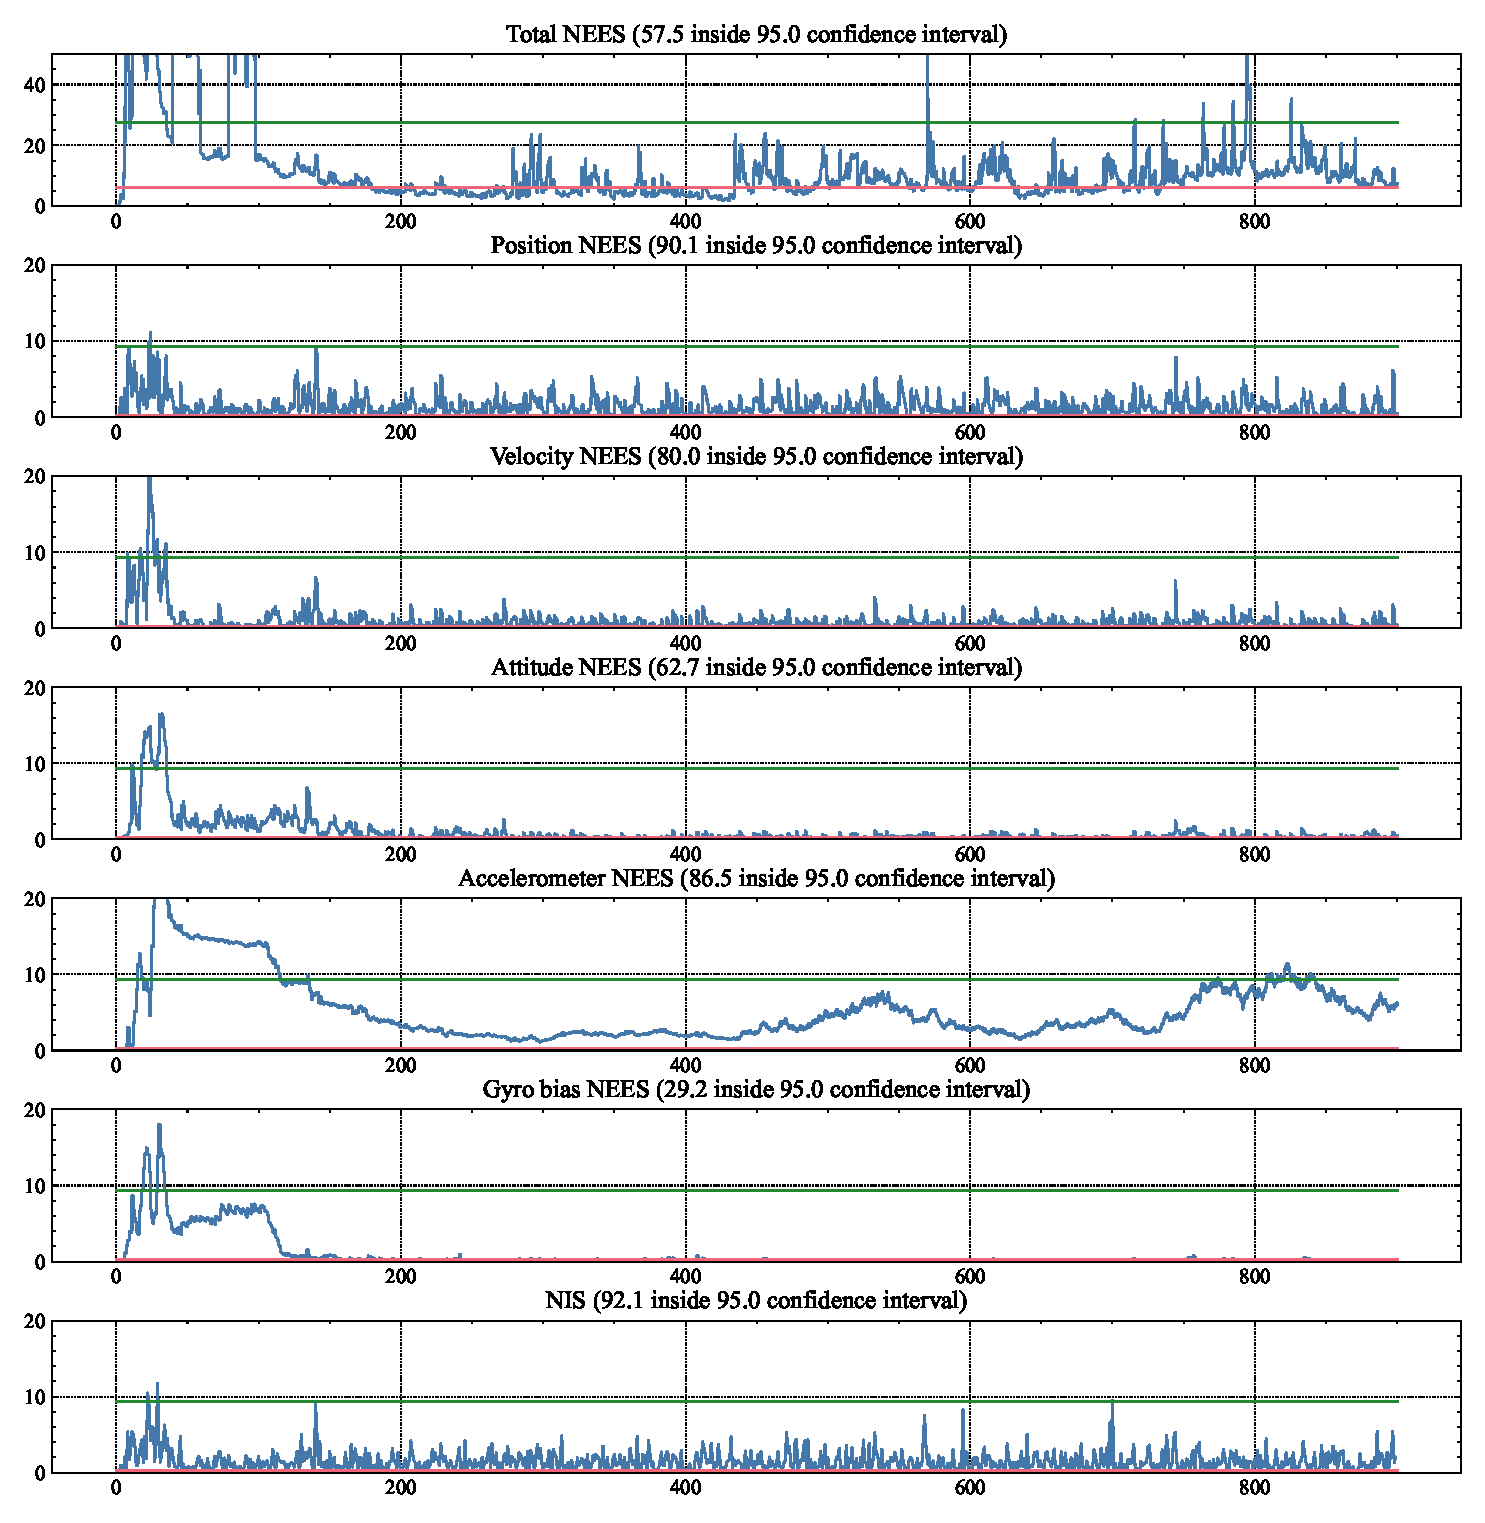
\includegraphics[clip, trim= 0cm 0cm 0cm 0cm, width = \textwidth]{figures/sim_5.eps}
    \caption{NEESes and NIS}
    \label{fig:23states}
\end{figure}
\begin{figure}
    \centering
    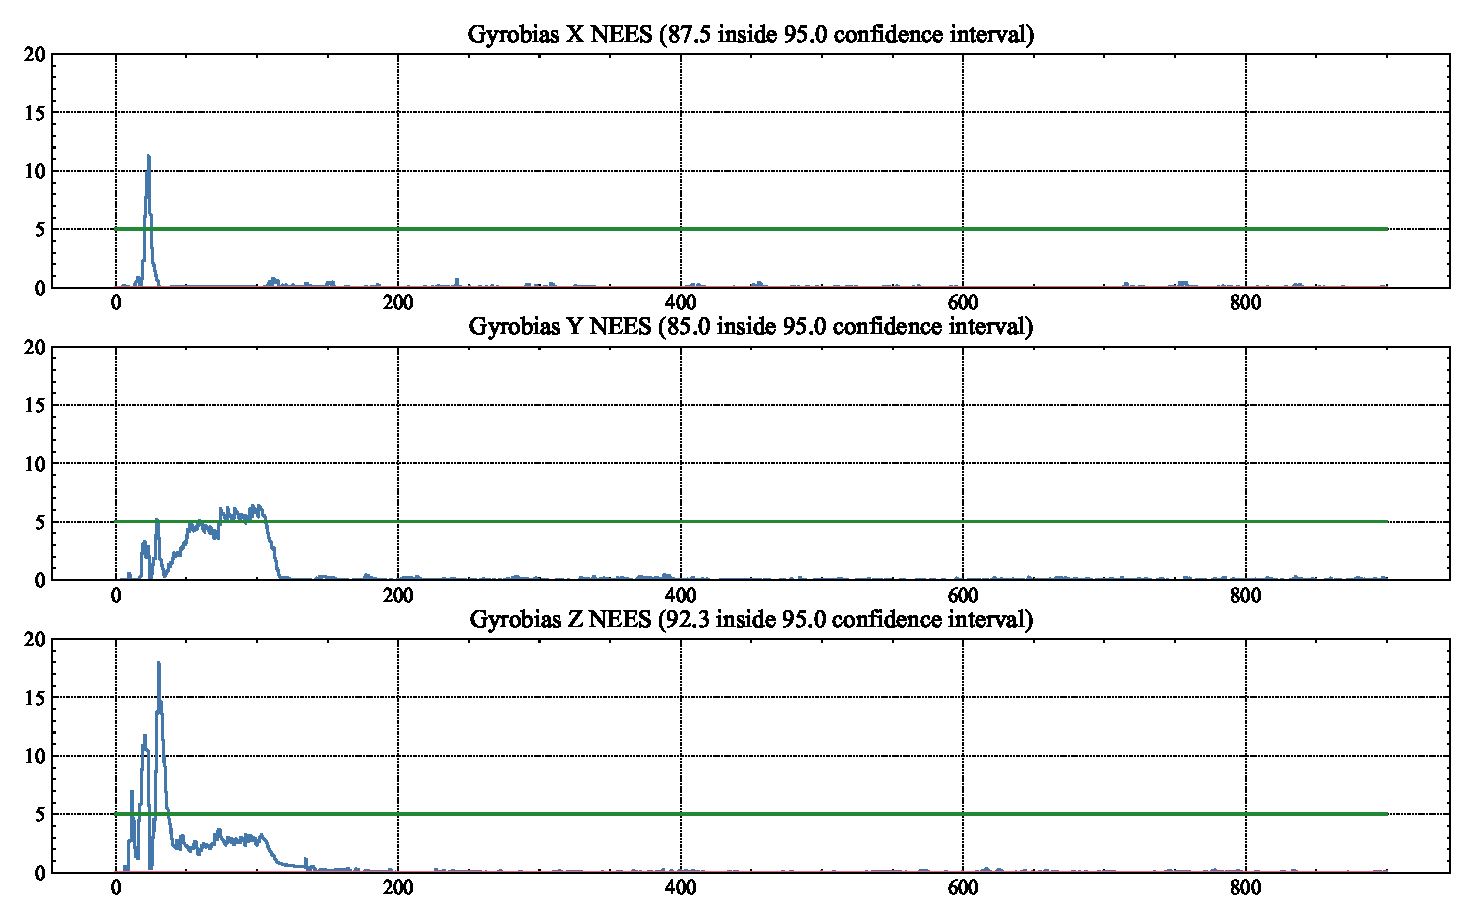
\includegraphics[clip, trim= 0cm 0cm 0cm 0cm, width = \textwidth]{figures/sim_8.eps}
    \caption{Assignment 2. Task 3. States}
    \label{fig:23states}
\end{figure}